% =============================================================================
% Efficient Multi-Tenant LoRA Serving for Encoder Models
% via Late-Fusion Batched Matrix Multiplication
%
% Target venue: EMNLP 2026 Industry Track (ACL-format, 6-page body limit;
%               Limitations / Ethics / References / appendix are excluded)
% Draft status: 2026-05-12
%   [DONE] Abstract, Introduction, Background, System Design, Related Work,
%          Limitations, Conclusion, verified BibTeX
%   [TODO] Baseline comparison table (task #2)
%   [TODO] Real-task accuracy evaluation (task #3)
%   [TODO] Multi-GPU × multi-model matrix (task #4)
%   [TODO] Statistical CI runs (task #6)
%   [TODO] Ablation table (task #7)
%   [TODO] Profile breakdown figure (task #11)
%   [TODO] Publication-quality figures (task #14)
% =============================================================================

\documentclass[11pt]{article}
\usepackage[preprint]{acl} % preprint: no line numbers, shows authors
% swap to \usepackage[review]{acl} before submission (adds line numbers, anonymises)
% swap to \usepackage{acl} for camera-ready

% ---- standard packages ----
\usepackage{times}
\usepackage{latexsym}
\usepackage[T1]{fontenc}
\usepackage[utf8]{inputenc}
\usepackage{microtype}
\usepackage{inconsolata}
\usepackage{amsmath}
\usepackage{amssymb}
\usepackage{booktabs}
\usepackage{multirow}
\usepackage{graphicx}
\usepackage{subcaption}
\usepackage{xcolor}
\usepackage[colorinlistoftodos,prependcaption]{todonotes}
% algorithm/algpseudocode: uncomment when pseudocode is added
% \usepackage{algorithm}
% \usepackage{algpseudocode}
\usepackage{hyperref}
\usepackage{url}
\usepackage{xspace}

% ---- consistent macros ----
\newcommand{\sysname}{LateFuse}
\newcommand{\ie}{i.e.,\xspace}
\newcommand{\eg}{e.g.,\xspace}
\newcommand{\etal}{\textit{et al.}\xspace}

% ---- todo macro styling ----
\newcommand{\todoinline}[1]{\todo[inline]{#1}}

% =============================================================================
\title{Efficient Multi-Tenant LoRA Serving for Encoder Models\\
       via Late-Fusion Batched Matrix Multiplication}

% Anonymized for double-blind review.
\author{Anonymous}

\begin{document}
\maketitle

% =============================================================================
\begin{abstract}
We introduce \sysname, a system for serving thousands of independently
fine-tuned LoRA adapters on a single shared encoder model in a single GPU
forward pass.
Personalizing an NLP feature (e.g.\ text classification) for thousands of
customers traditionally required one fine-tuned model per customer.
LoRA \cite{hu2022lora} eliminated the \emph{storage} barrier by reducing
per-customer state to a few hundred kilobytes; the remaining barrier is
\emph{serving}---batching requests across customers without merging adapter
weights into the base model.
\sysname{} avoids weight merging by computing the base projection
$W_0 x$ and the per-tenant LoRA delta $\Delta W_i x = B_i A_i x$ separately,
then fusing them additively---enabling heterogeneous adapters and per-tenant
logistic-regression heads to be batched via \texttt{torch.bmm} with
pre-allocated GPU buffers, requiring no custom CUDA kernels.
On a single NVIDIA A100-80GB GPU with \texttt{BAAI/bge-m3} as the base
model, \sysname{} serves \textbf{47{,}000 pre-loaded LoRA adapters at 810
samples/sec} with 41~ms p99 latency at batch size 32, and p50 latency stays
statistically unchanged from 100 to 47{,}000 adapters---the full per-GPU
capacity---empirically confirming $\mathcal{O}(1)$ scaling in adapter count.
Against the HuggingFace PEFT swap baseline on the same hardware,
\sysname{} delivers a \textbf{37--528$\times$ throughput improvement} under
adapter-grouped (batch-by-adapter) batching, growing with both batch size
and adapter pool size, plus a \textbf{$>$600$\times$ improvement in cold-start
deployment time}.
\end{abstract}

% =============================================================================
\section{Introduction}
\label{sec:intro}

Deploying a personalized NLP feature---such as text classification---to
thousands of customers is a storage and compute challenge.
Maintaining a fully fine-tuned model per customer is infeasible:
at $\approx$1.1~GB per copy in float16, serving 20{,}000 customers would require
over 22~TB of model weights.
LoRA \cite{hu2022lora} resolves the \emph{storage} problem: by expressing
each customer's adaptation as a low-rank update to a single shared base
encoder, the per-customer footprint shrinks to $\approx$1.6~MB (rank~8,
24 layers)---a $\approx$700$\times$ reduction.
The remaining challenge is \textbf{batched serving} across heterogeneous
adapters on a single GPU.

Existing multi-tenant LoRA serving systems---Punica \cite{chen2024punica},
S-LoRA \cite{sheng2024slora}, vLLM \cite{kwon2023vllm}, and LoRAX
\cite{predibase2023lorax}---target autoregressive decoder workloads, where
custom CUDA kernels and paged-memory pools are needed for token-by-token
generation over a KV cache. Encoders are structurally different: the
bidirectional forward pass at sequence length $S \gg 1$ is compute-bound
and dominated by base-model projections, so the LoRA path consumes only
$\approx$5\% of forward GPU time and any custom-kernel replacement is
bounded to single-digit speedup (\S\ref{sec:results_custom_kernels},
Finding~6). This makes standard batched matrix multiplication, rather
than a custom kernel, the right primitive. Heterogeneous-adapter
batching for encoder models is, to our knowledge, not yet supported by
released runtimes (\S\ref{sec:relwork}).

We present \sysname, a serving system that fills this gap.
The core insight is to fuse adapters in \emph{activation space} rather
than \emph{parameter space}: merging $B_i A_i$ into $W_0$ produces a
per-sample weight matrix $W'_i$ that must be applied serially, but
computing the base output $W_0 x$ and the delta $B_i A_i x$ separately
and summing them lets the per-sample work live inside a single batched
matrix multiplication. \sysname{} runs the shared base path once over
all $\mathcal{B}$ samples and dispatches the per-sample LoRA paths in
parallel via one \texttt{torch.bmm} call per attention layer, so a
mixed-tenant batch completes in a single forward pass regardless of how
many distinct adapters it references. Per-tenant task heads
(variable-size classifiers, regressors, retrieval re-rankers) are
batched analogously via zero-padded BMM.

Our single-GPU evaluation characterizes the serving primitive; a
minimal reference deployment for stateless scale-out is in
Appendix~\ref{sec:deployment}.

\paragraph{Contributions.}
\begin{itemize}
  \item We identify and formalize the \emph{encoder multi-tenant LoRA serving}
  problem, and show that existing systems leave it unsolved
  (\S\ref{sec:relwork}).

  \item We present late-fusion BMM serving, an architecture that batches
  arbitrary mixed-tenant encoder requests without weight merging and
  without custom CUDA kernels, in standard PyTorch (\S\ref{sec:system}).

  \item We empirically demonstrate that adapter count does not drive
  inference latency: scaling from 100 to 47{,}000 adapters at batch
  size 32 on a single A100-80GB leaves p50 latency flat
  (38.0$\to$38.3~ms) and p99 bounded ($\le$50.8~ms), with serving
  throughput saturating at $\approx$840~samples/sec by batch size 64
  (\S\ref{sec:experiments}).

  \item We benchmark \sysname{} against a HuggingFace PEFT swap baseline
  on identical hardware and show \textbf{37--528$\times$} throughput
  improvements under adapter-grouped batching and \textbf{$>$600$\times$}
  cold-start deployment improvements. By holding batch composition fixed
  and varying only $N$, we isolate \texttt{set\_adapter} as the
  $\mathcal{O}(N)$ bottleneck in the state-of-the-practice baseline
  (\S\ref{sec:results_baselines}, Finding~7).

  \item By staying in standard PyTorch, \sysname{} removes the custom-CUDA
  build step that is the dominant deployment friction on managed GPU
  platforms (Databricks, SageMaker, Modal), letting the same serving
  primitive drop into a standard cluster scale-out
  (Appendix~\ref{sec:deployment}).
\end{itemize}

% =============================================================================
\section{Background}
\label{sec:background}

\subsection{LoRA for Encoder Models}
\label{sec:background_lora}

LoRA \cite{hu2022lora} decomposes a weight update $\Delta W \in
\mathbb{R}^{d \times d}$ as the product of two low-rank matrices:
\begin{equation}
  \Delta W = B A, \quad
  A \in \mathbb{R}^{r \times d},\;
  B \in \mathbb{R}^{d \times r},\;
  r \ll d.
\end{equation}
The full forward pass for a single sample becomes
$h = W_0 x + \frac{\alpha}{r} B A x$,
where $W_0$ is the frozen pre-trained weight and $\alpha$ is a scaling
hyperparameter typically set equal to $r$.
For an encoder of hidden size $d = 1024$ with $L = 24$ layers, applying LoRA
at rank $r = 8$ to the query and value projections yields
$2 L \cdot (d r + r d) = 786{,}432$ trainable parameters per adapter---a
$64\times$ reduction over full fine-tuning of those layers.

In this work, $B$ is initialized to zero so that $\Delta W = 0$ at the start
of training, leaving the pre-trained representations intact.

At rank 8, LoRA retains $\approx$97\% of vanilla fine-tuning's mean
accuracy across seven public text-classification benchmarks
(Table~\ref{tab:accuracy}), at $1/370$ the trainable-parameter
cost.\footnote{Accuracy reported on
\texttt{paraphrase-mpnet-base-v2} to match the SetFit literature
\cite{tunstall2022efficient}; serving experiments
(\S\ref{sec:experiments}) use the larger \texttt{BAAI/bge-m3}
encoder.} The remaining barrier is \emph{serving}: combining thousands of
these adapters in a single forward pass.

\begin{table}[h]
\centering
\small
\caption{Per-task accuracy of LoRA adapters versus full encoder
fine-tuning at $N{=}8$ examples per class, rank=8, single seed on
\texttt{paraphrase-mpnet-base-v2}. LoRA retains $97\%$ of vanilla mean
accuracy at $1/370$ of the trainable parameter count. See
Appendix~\ref{app:accuracy} for per-task details.}
\label{tab:accuracy}
\begin{tabular}{lrrr}
\toprule
Dataset & Vanilla & LoRA-$r$8 & $\Delta$ \\
\midrule
SST-2          & 0.817 & 0.801 & $-$0.016 \\
SST-5          & 0.374 & 0.360 & $-$0.014 \\
CR             & 0.771 & 0.742 & $-$0.029 \\
Amazon-CF      & 0.568 & 0.563 & $-$0.005 \\
Emotion        & 0.361 & 0.310 & $-$0.051 \\
EnronSpam      & 0.890 & 0.884 & $-$0.006 \\
AG News        & 0.804 & 0.770 & $-$0.034 \\
\midrule
\textbf{Mean}  & \textbf{0.655} & \textbf{0.633} & $-$0.022 \\
Trainable params & 109M & 295K & 370$\times$ smaller \\
\bottomrule
\end{tabular}
\end{table}

\subsection{The Multi-Tenant Serving Problem}
\label{sec:background_serving}

Consider a service that exposes a single classification feature to $N$
customers, where each customer gets a fine-tuned
\texttt{BAAI/bge-m3} \cite{chen2024bge} on their own labeled
data to specialize the feature to their domain.
Three naive serving strategies all fail at scale.
\emph{One model per tenant} requires $N \times 1.1$~GB in float16
($\approx$22~TB at $N{=}20{,}000$, or $>$275 A100-80GBs of weight storage) and
admits no cross-tenant batching.
\emph{Weight merging per request}---compute $W' = W_0 + B_i A_i$ in-place,
run inference, then restore $W_0$---serializes requests behind the
merge--restore cycle, fragments GPU memory under in-place mutation, and
risks cross-tenant contamination if a crash interleaves with restore.
\emph{Sequential single-tenant batching} (one tenant per batch) drives
average GPU utilization toward $1/N$.
The right solution batches \emph{heterogeneous} adapters in a single forward
pass, which requires a decomposition where different linear operations can be
applied per sample without serialization.

% =============================================================================
\section{\sysname: System Design}
% * <Ashutosh Dwivedi> 18:25:09 26 May 2026 UTC+0530:
% Keshav : Section 5: Related work should be section 3. Section 3 : System Design should be section 5.
\label{sec:system}

% TODO (Task #14): Figure 1 — architecture diagram of the late-fusion
% forward pass. Should depict: (left) per-sample adapter stacking into
% batched B/A tensors; (center) split base path W0x and delta path BAx
% running in parallel; (right) element-wise fusion and LR head BMM.
% \begin{figure}[t]
%   \centering
%   \caption{Overview of late-fusion BMM serving in \sysname.
%     For a mixed-tenant batch of size $\mathcal{B}$, the base attention projection
%     $W_0 x$ runs once (shared weights), while per-sample LoRA deltas
%     $B_i A_i x$ are computed in two \texttt{torch.bmm} calls.
%     All $\mathcal{B}$ samples are fused in a single forward pass regardless of how many
%     distinct adapters are present.}
%   \label{fig:overview}
% \end{figure}

\subsection{Late-Fusion Decomposition}
\label{sec:lf_decomp}

The core insight is that the LoRA forward pass
$h = W_0 x + B_i A_i x$
can be split into two \emph{independent} computations:
\begin{align}
  h_{\text{base}} &= W_0 x \label{eq:base} \\
  h_{\text{delta}} &= B_i (A_i x) \label{eq:delta} \\
  h &= h_{\text{base}} + h_{\text{delta}} \label{eq:fuse}
\end{align}

Equation~\ref{eq:base} uses the same frozen $W_0$ for every sample in the
batch and is computed by standard PyTorch linear layers.
Equation~\ref{eq:delta} applies a \emph{different} $(A_i, B_i)$ pair to each
sample $i$, which requires batched matrix multiplication rather than a
broadcast multiply.
Equation~\ref{eq:fuse} is a zero-allocation element-wise addition.

For a batch of $\mathcal{B}$ samples with hidden size $H$ and sequence length $S$:
\begin{align}
  h_{\text{shrink}} &= \texttt{bmm}(x,\; [A_0,\ldots,A_{\mathcal{B}-1}])
    \in \mathbb{R}^{\mathcal{B} \times S \times r} \label{eq:shrink} \\
  h_{\text{delta}} &= \texttt{bmm}(h_{\text{shrink}},\; [B_0,\ldots,B_{\mathcal{B}-1}])
    \in \mathbb{R}^{\mathcal{B} \times S \times H} \label{eq:expand}
\end{align}

\noindent
where $[A_0, \ldots, A_{\mathcal{B}-1}] \in \mathbb{R}^{\mathcal{B} \times H \times r}$ is the
stack of per-sample shrink matrices, assembled from the adapter store at
request time.
Both \texttt{bmm} calls are a single GPU kernel launch, processing all $\mathcal{B}$
samples simultaneously regardless of how many distinct adapters they reference.

This decomposition contrasts with the SGMV kernel used in Punica
\cite{chen2024punica}: SGMV groups inputs by LoRA model ID and dispatches
per-group thread-blocks, whereas \texttt{torch.bmm} applies a distinct
$(A_i, B_i)$ to every batch item with no grouping; and SGMV operates on
vector inputs $(1, H)$ optimized for autoregressive decode, whereas
\texttt{bmm} operates on the $(S, H)$ matrix shape native to encoder
prefill. The concurrent S-LoRA \cite{sheng2024slora} introduces
prefill-shaped variants (MBGMM/MBGMV) over a paged adapter pool, but
still targets autoregressive LLM serving with a KV cache.

\subsection{Batched Classification Heads}
\label{sec:lr_head}

In the multi-tenant classification setting, each tenant trains a
% * <Ashutosh Dwivedi> 18:21:21 26 May 2026 UTC+0530:
% Kehsav : 1.⁠ ⁠Should we talk about Logistic Regression head or avoid it ?
logistic-regression (LR) head on top of the encoder's pooled
\texttt{[CLS]} representation.
Tenants differ in the number of output classes: tenant $i$ may have $c_i$
classes where $c_i$ varies from 2 to over 100.

\sysname{} serves all heads in a single BMM call.
Given a batch of pooled representations
$p \in \mathbb{R}^{\mathcal{B} \times 1 \times H}$
and per-tenant weight matrices
$W^{\text{cls}}_i \in \mathbb{R}^{c_i \times H}$ and bias vectors
$b^{\text{cls}}_i \in \mathbb{R}^{c_i}$,
we zero-pad all weight matrices to the maximum label count
$c_{\max} = \max_i c_i$ in the batch and form a stacked tensor
$W^{\text{cls}} \in \mathbb{R}^{\mathcal{B} \times c_{\max} \times H}$.
The logit computation is:
\begin{equation}
  \text{logits} = \texttt{bmm}(p,\; {W^{\text{cls}}}^\top) + b^{\text{cls}}
  \;\in\; \mathbb{R}^{\mathcal{B} \times 1 \times c_{\max}}
\end{equation}

Callers slice $[:, :, :c_i]$ per sample before applying softmax.
The zero-padded columns contribute zero gradient and do not affect the
probability distribution of any tenant.

\subsection{Implementation}
\label{sec:impl}

\paragraph{Pre-allocated buffers.}
A naive implementation lets \texttt{torch.bmm} allocate a fresh output
tensor on every call, producing $2 \times |\mathcal{M}| \times L$
allocations per forward pass (96 for $L{=}24$, $|\mathcal{M}|{=}2$). Each
invokes the CUDA caching allocator at microsecond cost, adding several
hundred microseconds of pure allocator overhead per batch.
\sysname{} instead pre-allocates two fixed-size buffers at initialization,
$\mathtt{out\_A} \in \mathbb{R}^{\mathcal{B}_{\max} \times S_{\max} \times r}$
and $\mathtt{out\_B} \in \mathbb{R}^{\mathcal{B}_{\max} \times S_{\max} \times H}$,
and passes them via the \texttt{out=} argument of every \texttt{bmm} call.
Both are shared across layers because each \texttt{expand} consumes
\texttt{out\_A} before the next \texttt{shrink} overwrites it.

\paragraph{Adapter store and batch assembly.}
At service startup, \sysname{} pre-loads all tenant LoRA adapters into GPU
memory as an \texttt{AdapterStore}: a dictionary mapping adapter IDs to
\texttt{LoraWeight} objects holding
$W_A \in \mathbb{R}^{L \times H \times r}$ and
$W_B \in \mathbb{R}^{L \times r \times H}$, stored in inference-transposed
layout so \texttt{bmm} requires no runtime transpose.
For a batch of adapter IDs, the \texttt{BatchAssembler} gathers each
adapter's per-layer $W_A$/$W_B$ slices into per-layer Python lists. This
CPU-side gather---a loop over samples, layers, and target modules---is the
dominant per-request overhead before the GPU forward pass
(\S\ref{sec:results_latency}). The per-layer lists are concatenated into
$(\mathcal{B}, H, r)$ and $(\mathcal{B}, r, H)$ tensors lazily inside the
forward, one \texttt{torch.cat} per layer immediately before its
\texttt{bmm}, so this concatenation is attributed to forward rather than
assembly time.

\subsection{Complexity Analysis}
\label{sec:complexity}

\paragraph{Memory.}
The base model requires $\mathcal{O}(d^2 L)$ memory regardless of tenant
count.
Each adapter requires $\mathcal{O}(r d L)$ memory.
For $N$ tenants: total GPU memory $= \mathcal{O}(d^2 L + N r d L)$.
At $d=1024$, $L=24$, $r=8$: 100 adapters occupy 157~MB; 20{,}000 adapters
occupy 31.5~GB.
An NVIDIA A100-80GB can hold $\approx$47{,}000 adapters at rank 8 before
exhausting memory.

\paragraph{Inference time.}
The latency of a single forward pass is independent of $N$ (adapter count):
it depends only on batch size $\mathcal{B}$, sequence length $S$, and model depth $L$.
The adapter count affects only CPU-side batch assembly time, which is
$\mathcal{O}(\mathcal{B} \cdot L \cdot |\mathcal{M}|)$ where $|\mathcal{M}|$ is the
number of target modules.
Empirically, increasing $N$ from 100 to 47{,}000 at batch size 32 leaves p50
latency effectively unchanged (38.0 vs.\ 38.3~ms;
\S\ref{sec:results_latency}).

% =============================================================================
\section{Experiments}
\label{sec:experiments}

\subsection{Setup}
\label{sec:setup}

\paragraph{Base model.}
Primary experiments use \texttt{BAAI/bge-m3} \cite{chen2024bge},
a 24-layer XLM-RoBERTa-derived encoder with hidden size $d=1024$,
16 attention heads, and $\approx$568M parameters.
This is among the most widely-served encoders for retrieval and classification
in production multi-tenant systems, and at $d=1024$ with $\approx$568M
parameters it is a demanding setting for the per-request overheads we measure.

\paragraph{LoRA configuration.}
We apply LoRA to the query and value projection matrices of each attention
layer (\texttt{target\_modules = [query, value]}).
We sweep rank $r \in \{4, 8, 16, 32\}$ with $\alpha = r$ (no scaling), matching
the configuration used by our PEFT-equivalence numerical tests.

\paragraph{Hardware.}
Primary experiments run on a single NVIDIA A100-SXM4-80GB GPU on a
cloud-managed node with PyTorch 2.11.0+cu128 in float16 precision.
We measure one node; the design scales out horizontally via stateless,
tenant-sticky replicas (reference Kubernetes deployment in
Appendix~\ref{sec:deployment}; not benchmarked).

\paragraph{Benchmark protocol.}
We measure end-to-end latency (batch assembly + encoder forward pass + LR head)
using 50 warm-up iterations followed by 200 measured iterations.
GPU-side work is timed with reusable \texttt{torch.cuda.Event} pairs and
synchronized once per iteration; CPU-side assembly is timed with
\texttt{time.perf\_counter} between identical synchronization points.
We sweep adapter count $N \in \{100,\,1{,}000,\,5{,}000,\,10{,}000,\,20{,}000,\,40{,}000,\,47{,}000\}$,
batch size $\mathcal{B} \in \{8,\,16,\,32,\,64,\,128\}$, and rank
$r \in \{4,\,8,\,16,\,32\}$.
Each configuration samples mixed-tenant batches uniformly at random from the
adapter pool.

\paragraph{Adapters and correctness.}
Latency and throughput experiments use synthetic LoRA weights, isolating
serving-system overhead from adapter-quality artefacts. We numerically
verify that \sysname{}'s output is bit-equivalent to a reference
PEFT-wrapped \texttt{AutoModel} with the same A/B weights to within
\texttt{atol=rtol=1e-4} in fp32 across five scenarios---zero-LoRA, single
shared adapter, per-sample distinct adapters with shared per-layer A/B,
per-target-module distinct A/B, and a padded XLM-RoBERTa batch exercising
the \texttt{bge-m3} positional scheme---each enforced as a unit test, covering
both the BERT and XLM-RoBERTa position-id conventions.

\paragraph{Baselines.}
We compare against \texttt{HuggingFace PEFT}~\cite{mangrulkar2022peft} in an
adapter-grouped configuration (\S\ref{sec:results_baselines}).
\texttt{vLLM} \cite{kwon2023vllm} supports single-adapter encoder LoRA as of
v0.8.3 but does not yet support multi-adapter classification serving
(in-progress PR~\#24596, unmerged as of submission);
\texttt{LoRAX} \cite{predibase2023lorax} is likewise decoder-oriented.
We therefore omit these from quantitative comparison; see
\S\ref{sec:relwork} for a detailed discussion.

\subsection{Latency and Throughput Scaling}
\label{sec:results_latency}

Table~\ref{tab:main_results} reports p50/p90/p99 latency and throughput
across a one-factor-at-a-time sweep of this space, varying $N$, $\mathcal{B}$,
and $r$ in turn around the $N{=}1{,}000$, $\mathcal{B}{=}32$, $r{=}8$
operating point.

\begin{table}[t]
\centering
\small
\setlength{\tabcolsep}{4.5pt}
\renewcommand{\arraystretch}{0.92}
\caption{Serving latency, throughput, and peak GPU memory
(\texttt{BAAI/bge-m3}, A100-SXM4-80GB; full setup in \S\ref{sec:setup}).
Adapters are pre-loaded; latency includes batch assembly and the
classification head. The top block sweeps adapter count, the middle
batch size, and the bottom LoRA rank.}
\label{tab:main_results}
\begin{tabular}{rrr rrr r r}
\toprule
$N$ & $\mathcal{B}$ & $r$ & p50 & p90 & p99 & QPS & GPU \\
    &     &     & (ms)& (ms)& (ms)& (s/s) & (GB) \\
\midrule
    100 & 32 & 8  & 38.0 & 38.2 & 42.4 & 816 & 1.43 \\
  1{,}000 & 32 & 8  & 38.0 & 38.2 & 39.0 & 827 & 2.87 \\
  5{,}000 & 32 & 8  & 38.2 & 38.4 & 50.8 & 794 & 9.24 \\
 10{,}000 & 32 & 8  & 38.2 & 38.4 & 44.9 & 806 & 17.21 \\
 20{,}000 & 32 & 8  & 38.3 & 38.4 & 38.8 & 836 & 33.15 \\
 40{,}000 & 32 & 8  & 38.3 & 38.5 & 42.4 & 783 & 65.03 \\
 47{,}000 & 32 & 8  & 38.3 & 38.5 & 40.8 & 807 & 76.18 \\
\midrule
  1{,}000 & 8  & 8  & 20.1 & 20.3 & 20.5 & 399 & 2.77 \\
  1{,}000 & 16 & 8  & 23.2 & 23.3 & 23.6 & 688 & 2.80 \\
  1{,}000 & 64 & 8  & 72.0 & 72.4 & 196.5 & 844 & 3.00 \\
  1{,}000 & 128& 8  & 140.8 & 141.9 & 264.1 & 843 & 3.25 \\
\midrule
  1{,}000 & 32 & 4  & 39.2 & 39.4 & 41.1 & 789 & 2.08 \\
  1{,}000 & 32 & 16 & 39.0 & 39.1 & 40.5 & 820 & 4.44 \\
  1{,}000 & 32 & 32 & 39.1 & 39.1 & 39.2 & 819 & 7.75 \\
\bottomrule
\end{tabular}
\end{table}

\paragraph{Finding 1: Adapter count does not drive latency.}
Scaling from 100 to 47{,}000 adapters at $\mathcal{B}{=}32$, $r{=}8$ leaves p50 latency
statistically unchanged (38.0 vs.\ 38.3~ms, 0.8\%)---a 470$\times$ increase in
served customers at zero latency cost, sustained to the per-GPU memory ceiling
(Finding~4).
The GPU-side forward pass time is constant at $\approx$25.8~ms across the
entire sweep, and the only $N$-dependent component is the CPU-side batch
assembler, whose share stays below 38\% of total latency---empirically
validating the $\mathcal{O}(1)$-in-$N$ scaling of \S\ref{sec:complexity}.

\paragraph{Finding 2: Batch size drives throughput up to saturation at $\mathcal{B}{=}64$.}
Throughput scales from 399~samples/sec at $\mathcal{B}{=}8$ to 844~samples/sec at
$\mathcal{B}{=}64$, then plateaus---$\mathcal{B}{=}128$ delivers no further gain (843~samples/sec).
The shared-base encoder forward becomes GPU-bound at $\mathcal{B}{=}64$, after which
larger batches only widen tail latency without lifting throughput, making
$\mathcal{B} \in \{32, 64\}$ the recommended range under strict p99 SLAs.

\paragraph{Finding 3: LoRA rank is a free latency knob in the small-rank regime.}
At $N{=}1{,}000$, $\mathcal{B}{=}32$, p50 latency is flat across $r \in \{4, 8, 16, 32\}$
(39.2, 39.0, 39.0, 39.1~ms respectively), with no rank trend in the tail either
(p99 = 41.1, 40.8, 40.5, 39.2~ms). While $r \ll H$, the low-rank path adds only
$2r/H$ of a base projection's arithmetic ($\approx$1\% of the full encoder
forward), so the per-batch GPU forward stays at $\approx$26~ms across all four
ranks; the knob ceases to be free once $2r$ approaches $H$.
Within this regime, rank is a pure quality--memory tradeoff: doubling it leaves
forward latency unchanged but doubles the per-adapter footprint, halving the
per-GPU tenant ceiling ($\approx$47{,}000 adapters at $r{=}8$ versus
$\approx$12{,}000 at $r{=}32$; Finding~4).

\paragraph{Finding 4: Predictable memory footprint and per-GPU ceiling.}
Per-adapter cache memory measures 1.573~MB at $r{=}8$ in fp16 (24 layers,
hidden size 1024, two target modules), matching the analytic formula
$2 \cdot M \cdot L \cdot d \cdot r \cdot \text{dtype}$ within 5\%.
On an 80~GB A100, after reserving $\approx$2~GB for base-model parameters and
activation buffers, this yields a clean empirical ceiling of
$\approx$\textbf{47{,}000} adapters at $r{=}8$ (the largest pool we verified,
occupying 76.2~GB), $\approx$\textbf{23{,}000} at
$r{=}16$, and $\approx$\textbf{12{,}000} at $r{=}32$.
Our $N{=}50{,}000$ runs OOM'd cleanly at all batch sizes, confirming the limit.

\paragraph{Finding 5: Batch assembly is the residual bottleneck and drives tail latency.}
\label{sec:results_assembly}
The CPU-side batch-assembly path (gather per-sample LoRA slices into
per-layer lists, pad the LR head, host-to-device copy) consumes 15.5\% of iteration time at $\mathcal{B}{=}8$
and \textbf{40\%} at $\mathcal{B}{=}128$, scaling linearly with $\mathcal{B}$
while the encoder forward saturates at $\mathcal{B}{=}64$.
This same path drives tail latency: the p99/p50 ratio is $1.03\times$ at
$\mathcal{B}{=}32$ but reaches $2.73\times$ at $\mathcal{B}{=}64$, with
profiling localizing the spike to occasional Python/GC stalls during
assembly; the GPU forward exhibits no such variance.
Double-buffered H2D transfer and a GPU-resident \texttt{index\_select} gather
would amortize this; both are future work.

\paragraph{Finding 6: Custom LoRA kernels offer only single-digit upside on
encoders.}
\label{sec:results_custom_kernels}
Could custom kernels (Punica's SGMV \cite{chen2024punica}, S-LoRA's MBGMV
\cite{sheng2024slora}) replacing our \texttt{torch.bmm} help? Three measurements
at $\mathcal{B}{=}32$, $N{=}1{,}000$, $r{=}8$ bound the upside to single digits. The \emph{analytic FLOP ratio} per layer is
$3d/r{=}384$, so even an instantaneous LoRA kernel saves at most $0.26\%$ of
FLOPs. A \emph{profiler trace} (self CUDA time, isolating the LoRA shrink/expand
via an apply-LoRA on/off difference) attributes \textbf{5.0\%} of forward GPU time
to the LoRA \texttt{bmm} versus \textbf{50.2\%} for the base projections. A
\emph{no-LoRA ablation} skipping the entire LoRA path (gather, shrink/expand,
merge) saves \textbf{2.2~ms of 26.0~ms} (\textbf{8.3\%}); the gather and merge,
not the \texttt{bmm}, dominate the gap above the $5.0\%$ kernel cost. Custom fused
kernels target only this path, so $8.3\%$ is the hard ceiling here---unlike
memory-bound decoder decode, where LoRA carries far higher relative weight and
custom kernels yield the multiplicative gains reported in that literature.

\begin{figure}[t]
  \centering
  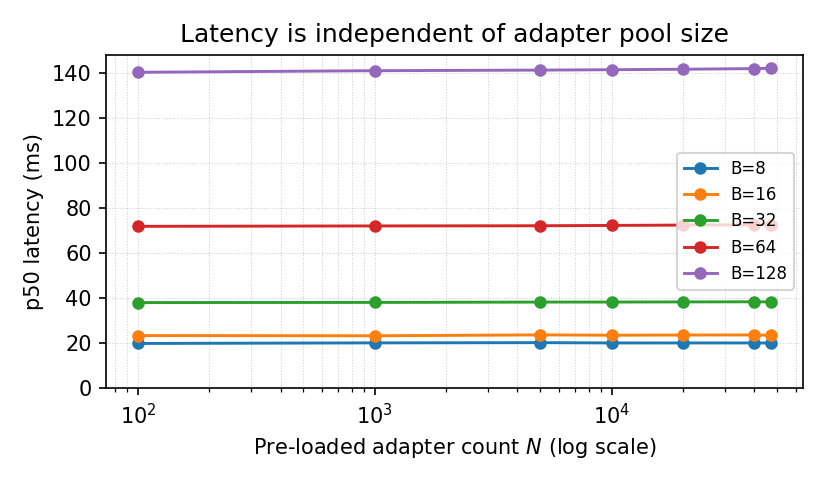
\includegraphics[width=0.52\linewidth]{figures/latency_adapters.png}
  \caption{p50 latency as a function of pre-loaded adapter count at five
  batch sizes (rank = 8, sequence length = 128, A100-80GB,
  \texttt{BAAI/bge-m3}).
  Curves are flat across $N \in [100, 47{,}000]$, empirically confirming the
  $\mathcal{O}(1)$-in-$N$ scaling property of \sysname.}
  \label{fig:latency_adapters}
\end{figure}

% Throughput-vs-baselines figure dropped: redundant with Table tab:baselines.
% \begin{figure}[t]
%   \centering
%   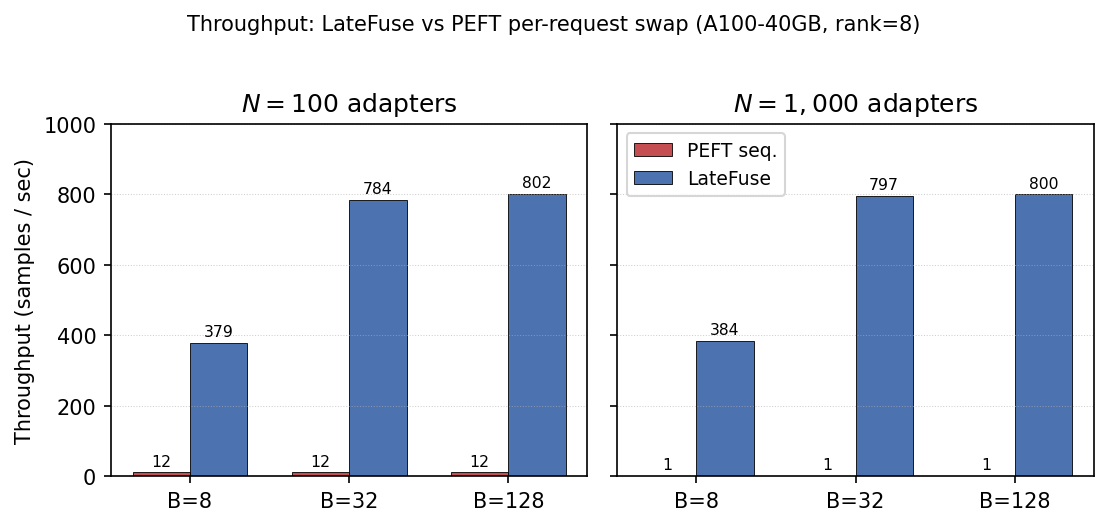
\includegraphics[width=\linewidth]{figures/throughput_baselines.png}
%   \caption{Throughput of \sysname{} versus the PEFT per-request swap baseline
%   at three batch sizes for $N \in \{100, 1{,}000\}$ adapters (rank = 8, fp16,
%   A100-40GB).
%   PEFT's throughput is invariant in $B$ (each sample requires its own
%   \texttt{set\_adapter}+forward) and collapses 8.4$\times$ as $N$ grows from
%   100 to 1{,}000.}
%   \label{fig:throughput_baselines}
% \end{figure}

\subsection{Comparison with Baselines}
\label{sec:results_baselines}

We compare against \texttt{HuggingFace PEFT} \cite{mangrulkar2022peft} in three
configurations, all attaching $N$ adapters via \texttt{add\_adapter}.
\emph{Grouped} buckets a mixed batch by adapter id, running one
\texttt{set\_adapter} and forward per bucket (Punica's SGMV strategy
\cite{chen2024punica}). \emph{Homogeneous}, PEFT's friendliest case, uses
single-tenant batches---one \texttt{set\_adapter} and one batched forward each.
\emph{Base} is the bare model with no adapters (702/1{,}810/2{,}067~samples/sec
at $\mathcal{B}{=}8/32/128$, $N$-independent). We also report PEFT's
$N$-adapter registration cost, which we replace with a constant-time
\texttt{AdapterStore} insert.

\begin{table}[h]
\centering
\footnotesize
\setlength{\tabcolsep}{4.5pt}
\renewcommand{\arraystretch}{0.95}
\caption{Latency and throughput vs.\ the PEFT swap baseline in its
\emph{grouped} (batch-by-adapter) and \emph{homogeneous} (single-tenant
batches, the friendliest case for PEFT) configurations (\texttt{BAAI/bge-m3},
A100-SXM4-80GB, rank=8; setup in \S\ref{sec:setup}). Grouped and \sysname{}
draw uniform mixed-tenant batches; the $N$-independent no-adapter base ceiling
is reported in-text. Speedup is \sysname{} over PEFT grouped.}
\label{tab:baselines}
\begin{tabular}{lrrrr}
\toprule
 & \multicolumn{2}{c}{$N = 100$} & \multicolumn{2}{c}{$N = 1{,}000$} \\
\cmidrule(lr){2-3} \cmidrule(lr){4-5}
System & p50 (ms) & QPS & p50 (ms) & QPS \\
\midrule
PEFT grouped ($\mathcal{B}{=}8$)      & 624  & 12.9 & 5{,}331  & 1.5 \\
PEFT grouped ($\mathcal{B}{=}32$)     & 2{,}085 & 15.1 & 20{,}865 & 1.5 \\
PEFT grouped ($\mathcal{B}{=}128$)    & 5{,}674 & 22.4 & 81{,}025 & 1.6 \\
\midrule
PEFT homog. ($\mathcal{B}{=}8$)    & 77  & 103  & 668 & 11.9 \\
PEFT homog. ($\mathcal{B}{=}32$)   & 82  & 390  & 670 & 47.5 \\
PEFT homog. ($\mathcal{B}{=}128$)  & 125 & 1{,}019 & 724 & 176 \\
\midrule
\sysname{} ($\mathcal{B}{=}8$)        & 20.6 & 384 & 20.7 & 368 \\
\sysname{} ($\mathcal{B}{=}32$)       & 38.5 & \textbf{810} & 38.7 & \textbf{792} \\
\sysname{} ($\mathcal{B}{=}128$)      & 143.2 & \textbf{828} & 144.1 & \textbf{825} \\
\midrule
\textbf{Speedup} ($\mathcal{B}{=}32$) & \multicolumn{2}{c}{\textbf{54$\times$}}
                            & \multicolumn{2}{c}{\textbf{528$\times$}} \\
\textbf{Speedup} ($\mathcal{B}{=}128$)& \multicolumn{2}{c}{\textbf{37$\times$}}
                            & \multicolumn{2}{c}{\textbf{516$\times$}} \\
\bottomrule
\end{tabular}
\end{table}

\paragraph{Finding 7: PEFT's per-swap cost is $\mathcal{O}(N)$ in the tenant pool.}
\emph{Homogeneous} batching---PEFT's best case (single-tenant batches, one
\texttt{set\_adapter} and forward each)---is competitive at $N{=}100$, even
edging \sysname{} at $\mathcal{B}{=}128$ (1{,}019 vs.\ 828~samples/sec). Yet
holding batching fixed and growing the pool to 1{,}000 collapses throughput
6--9$\times$ (390$\to$48~samples/sec at $\mathcal{B}{=}32$), leaving \sysname{}
5--31$\times$ faster; since only the adapter \emph{count} changed, this isolates
\texttt{set\_adapter} as $\mathcal{O}(N)$. \emph{Grouped} fares worse---mixed
batches rarely share an adapter, so \sysname{} leads by 54--528$\times$ at
$\mathcal{B}{=}32$.

% TODO (Task #4): §4.5 Multi-Model and Multi-Hardware Generalization.
% Run the latency/throughput sweep on at least 3 base encoders × 3 GPU classes:
%   Base encoders: bert-base-uncased (d=768, 12 layers),
%                  intfloat/multilingual-e5-base (d=768),
%                  intfloat/multilingual-e5-large (d=1024, 24 layers).
%   GPU classes:  NVIDIA T4 (16 GB, $0.40/hr), L4 (23 GB, $0.39/hr),
%                 A100-40GB ($1.10/hr).
% Report whether the O(1) adapter scaling property holds across model and
% GPU dimensions.
% \subsection{Multi-Model and Multi-Hardware Generalization}
% \label{sec:results_generalization}

% TODO (Task #7): §4.6 Ablation Study.
% Run ablations and fill in Table tab:ablation.
% Expected: buffer pre-allocation saves ~0.5 ms; contiguous A-matrix layout
% saves ~0.1–0.3 ms; float16 reduces memory 2× with 10–20% latency reduction.
% \subsection{Ablation Study}
% \label{sec:ablation}
%
% \begin{table}[h]
% \centering
% \small
% \caption{Ablation study: contribution of each design choice
% (20{,}000 adapters, batch=32, rank=8). TODO: fill in after Task #7.}
% \label{tab:ablation}
% \begin{tabular}{lrr}
% \toprule
% Configuration & p50 (ms) & $\Delta$ vs.\ full \\
% \midrule
% Full \sysname{}                                    & 56.3          & --- \\
% w/o pre-allocated buffers (dynamic alloc)          & \emph{?} & $+$\emph{?} \\
% w/o contiguous A-matrix layout (runtime transpose) & \emph{?} & $+$\emph{?} \\
% Query only (not query$+$value)                     & \emph{?} & $-$\emph{?} \\
% Query$+$Key$+$Value$+$Output                       & \emph{?} & $+$\emph{?} \\
% float16 precision                                  & \emph{?} & $-$\emph{?} \\
% \bottomrule
% \end{tabular}
% \end{table}

% =============================================================================
\section{Related Work}
\label{sec:relwork}

\paragraph{Multi-tenant LoRA serving for decoder LLMs.}
Punica \cite{chen2024punica} (SGMV, a custom CUDA kernel grouping a batch by
LoRA id for per-group matrix-vector products) and S-LoRA \cite{sheng2024slora}
(a paged memory pool with Triton MBGMM/MBGMV kernels for heterogeneous ranks)
both scope their designs to the autoregressive prefill$\to$decode pipeline and
never expose the encoder operations---bidirectional attention, pooling,
classification heads---that classification workloads require. vLLM
\cite{kwon2023vllm} adopts these kernels as its multi-LoRA backend, but
multi-adapter classification serving---the scope we target---was still unmerged
at submission (PR~\#24596). LoRAX \cite{predibase2023lorax}, MixLoRA
\cite{PLACEHOLDER_mixlora2024}, CaraServe \cite{su2023caraserve}, and dLoRA
\cite{wu2024dlora} likewise optimize decoder-only serving and do not address
encoder classifiers, variable-size classification heads, or deployment without
custom CUDA compilation.

\paragraph{Encoder and multi-adapter serving.}
HuggingFace TEI \cite{huggingface2023tei} serves encoder/embedding models at
high throughput via Flash Attention and cuBLASLt but has no adapter support.
PetS \cite{zhou2022pets}, the closest prior system, targets multi-adapter
encoder serving for Adapter \cite{houlsby2019adapter}, BitFit
\cite{benzaken2022bitfit}, and MaskBERT \cite{zhao2020masking} on
BERT/DistilBERT, but predates LoRA and handles neither low-rank decompositions
nor per-tenant classification heads.
\sysname{} is a LoRA-native framework that batches arbitrary external
adapters---with variable classification heads and a pre-loaded cache---without
modifying the base model.

% =============================================================================
\section{Conclusion}
\label{sec:conclusion}

We presented \sysname, a serving system for multi-tenant LoRA on encoder
models. Late-fusion batched matrix multiplication fuses the frozen base path
and per-tenant LoRA deltas additively, enabling mixed-tenant batches without
weight merging, custom CUDA kernels, or KV-cache machinery. In standard
PyTorch it serves 47{,}000 adapters on one A100-80GB at constant latency---a
$37$--$528\times$ gain over PEFT swapping.

% =============================================================================
\section*{Limitations}

\paragraph{Uniform rank constraint.}
All adapters in a batch must share the same rank $r$ and the same set of
target modules.
Serving tenants with heterogeneous fine-tuning strategies requires padding
every adapter to the maximum rank present in the batch, wasting compute on
low-rank adapters; a masked-BMM variant that avoids this padding overhead
remains future work.
% TODO (Task #8): mixed-rank experiment, finalize this paragraph after.

\paragraph{Pre-loaded adapter cache.}
\sysname{} holds all adapters in GPU memory permanently.
For workloads with more than $\sim$16{,}000 adapters at rank 8 on an L4, an
LRU eviction policy with CPU offload would be required.
Paged adapter storage analogous to PagedAttention
\cite{kwon2023vllm} is a natural extension.

\paragraph{CPU-side batch assembly.}
The \texttt{BatchAssembler} runs on CPU and gathers per-sample adapter
slices into per-layer lists via Python loops.
For very high request rates ($>$10{,}000 requests/sec), this becomes the
throughput bottleneck.
A custom CUDA or C++ gather kernel that indexes directly into the adapter
store would eliminate this overhead, at the cost of departing from
pure-PyTorch deployability.

\paragraph{Single-node evaluation.}
All latency and throughput results are measured on one GPU. The architecture
targets horizontal scale-out via stateless, tenant-sticky replicas, with a
reference Kubernetes deployment provided (Appendix~\ref{sec:deployment});
cluster-level throughput and behaviour under skewed (hot-tenant) traffic remain
to be evaluated.

\paragraph{Single-seed evaluation.}
Current benchmarks use a single random seed, so statistical significance is
not yet established.
% TODO (Task #6): multi-seed CI runs before camera-ready.

% =============================================================================
\section*{Ethics Statement}

This work addresses inference-time efficiency for multi-tenant NLP systems.
We identify no specific ethical concerns beyond those inherent to the
underlying models (\eg bias in pre-trained encoders).
The system is intended for legitimate multi-tenant SaaS deployments.
Adapter isolation is enforced by design: per-tenant weights are never merged
into the shared base model, eliminating cross-tenant contamination risks
present in weight-merging approaches.

% =============================================================================
\bibliography{references}

\appendix

% =============================================================================
\section{Per-Task Accuracy Details}
\label{app:accuracy}

Table~\ref{tab:accuracy} (\S\ref{sec:background_lora}) summarizes
LoRA-vs-vanilla classification accuracy across seven public benchmarks
used by the SetFit literature \cite{tunstall2022efficient}: SST-2,
SST-5, CR, Amazon-Counterfactual, Emotion, EnronSpam, and AG News. For
each dataset we train two variants of \texttt{paraphrase-mpnet-base-v2}
\cite{reimers2019sentencebert} at $N{=}8$ labeled examples per class: a
\emph{vanilla} full-encoder fine-tune (109M trainable parameters) and a
\emph{LoRA} variant at rank~8 (294{,}912 trainable parameters---a
$370\times$ reduction).

LoRA loses 2.2~percentage points of average accuracy in exchange for
the $370\times$ reduction in trainable parameters per tenant, which
translates directly into the per-adapter storage and GPU-cache footprint
reported in \S\ref{sec:results_latency}. The gap is smallest on tasks
dominated by the pretrained representation (EnronSpam: $-$0.6pp;
Amazon-CF: $-$0.5pp) and largest on tasks that benefit most from deep
encoder updates (Emotion: $-$5.1pp). For deployments where this gap is
unacceptable, rank can be increased at zero latency cost
(Finding~3); the only price is GPU memory.

% =============================================================================
\section{Horizontal Deployment}
\label{sec:deployment}

Our measurements isolate a single GPU node; this appendix describes how the
same serving primitive composes into a horizontally scaled cluster. We provide
a reference deployment---Kubernetes manifests and a FastAPI serving layer---that
is intentionally minimal: it demonstrates the architecture rather than
optimizing it, and is meant to be adapted to a given workload's batching,
autoscaling, and adapter-placement policy. We do not evaluate it empirically.

\paragraph{Stateless replicas.}
The base encoder is replicated across pods and adapters are loaded from
S3-compatible object storage, so the only per-node state is the in-GPU adapter
cache, which is reconstructible from storage. Each pod runs the dynamic batcher
and \sysname{} engine of \S\ref{sec:system} unchanged.

\paragraph{Tenant-sticky routing.}
An ingress layer routes by a consistent hash of the tenant identifier
(NGINX \texttt{upstream-hash-by} on an \texttt{X-Tenant-Id} header, mirrored by
an application-level hash ring with virtual nodes). Each tenant is thus pinned
to a single pod that holds its adapter resident in GPU memory, so the
$\mathcal{O}(1)$-in-$N$ latency we measure holds at each pod, and because the
replicas are independent, aggregate request throughput grows with the number of
pods ($\approx\!K\times$ a single node for $K$ pods). Serving more than a single
node's $\approx$47{,}000-adapter ceiling (Finding~4) additionally requires
partitioning the adapters across pods by the same hash, so each loads only its
shard; the reference deployment instead replicates a fixed adapter set per
pod---simpler, and adequate when the population fits one node---leaving
shard-aware placement as a configuration change.

\paragraph{Elasticity and hot reload.}
A horizontal pod autoscaler adds or removes replicas on utilisation metrics.
Consistent hashing remaps only $\approx\!1/K$ of tenants on a scaling event, so
disruption is bounded to those tenants, whose adapters are then (re)loaded on
their new pod from object storage. Adapter retraining is propagated by a
publish/subscribe channel (Redis) that triggers in-place reload without a pod
restart.

\paragraph{Routing caveat.}
Sticky routing pins a tenant to one pod, so a single high-traffic tenant cannot
be spread across nodes without sacrificing cache locality; cluster behaviour
under skewed tenant traffic is left to future work.

\end{document}
